\apendice{Especificación de Requisitos}

\section{Introducción}

En este apartado vamos a hablar sobre la planificación seguida en este trabajo, sus objetivos generales y sus requisitos.

\section{Objetivos generales}

El objetivo principal del trabajo era trabajar sobre la idea de la domótica y la posibilidad de manejar tu casa desde tu teléfono. Partiendo de esa base y realizando una estrategia \textit{Top-down}, entre mi tutor y yo realizamos unos objetos generales que este proyecto debería cumplir.

\begin{enumerate}
	\item Definir una habitación y los elementos a controlar.
	\item Conexión con la estación.
	\item Incremento de la funcionalidad de la aplicación.
	\item Desarrollo de la interfaz en la Raspberry Pi.
	\item Mejora de utilización de la aplicación.
	\item Lanzamiento de la primera versión completamente funcional.
	\item Documentación: Escribir memoria y anexos.
	\item Diseñar el póster de la presentación.
\end{enumerate}

\section{Catalogo de requisitos}

A partir de dichos objetivos y entrando más en detalle, se han obtenido los requisitos funcionales más generales según las ventanas con las que puede interactuar el usuario en la aplicación y en la Raspberry Pi.

\subsection{Requisitos funcionales para la aplicación}

\begin{figure}[h!]
	\centering
	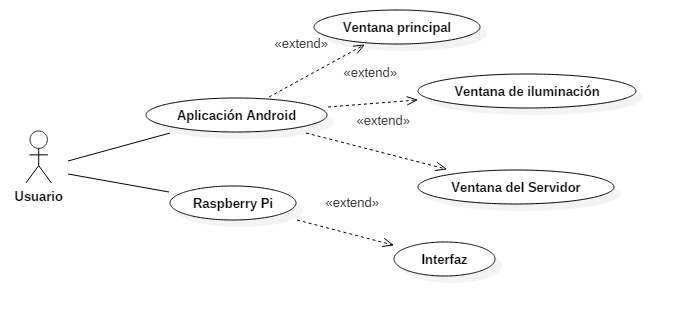
\includegraphics[width=1.2\linewidth]{img/CDUGeneral}
	\caption{Diagrama de casos de uso general.}
	\label{fig:CDUGeneral}
\end{figure}

\subsubsection{Ventana principal}

\begin{enumerate}
	\item Crear estancia.
	\item Modificar nombre.
	\item Eliminar estancia.
	\item Borrar base de datos.
	\item Ir a la ventana del Servidor. 
\end{enumerate}

\subsubsection{Ventana de Iluminación}

\begin{enumerate}
	\item Crear bombilla.
	\item Modificar nombre.
	\item Eliminar bombilla.
	\item Encender bombilla.
	\item Apagar bombilla.
	\item Volver a la ventana principal. 
\end{enumerate}

\subsubsection{Ventana del Servidor}

\begin{enumerate}
	\item Modificar IP
	\item Modificar Puerto.
	\item Conectar al servidor.
	\item Desconectar del servidor.
	\item Volver a la ventana principal.
\end{enumerate}

\subsubsection{Interfaz Raspberry}

\begin{enumerate}
	\item Actualizar IP.
\end{enumerate}

\section{Especificación de requisitos}

En este apartado, una vez hemos visto el diagrama de caso de uso general \ref{fig:CDUGeneral}, vamos a desglosarlo en diagramas de caso de uso más pequeños, \ref{fig:CDUVentanaPrincipal}, \ref{fig:CDUVentanaIluminacion}, \ref{fig:CDUVentanaServidor} y \ref{fig:CDUInterfazPython} que además contienen los requisitos funcionales nombrados en el punto anterior. Además, en las tablas \ref{tabla:CrearEstancia}, \ref{tabla:ModificarNombreEstancia}, \ref{tabla:EliminarEstancia}, \ref{tabla:BorrarBaseDeDatos}, \ref{tabla:ventanaServidor}, \ref{tabla:CrearBombilla}, \ref{tabla:ModificarNombreBombilla}, \ref{tabla:EliminarBombilla}, \ref{tabla:EncenderBombilla}, \ref{tabla:ApagarBombilla}, \ref{tabla:volverVentanaPrincipal}, \ref{tabla:ModificarIP}, \ref{tabla:ModificarPuerto}, \ref{tabla:ConectarAlServidor}, \ref{tabla:DesconectarDelServidor}, \ref{tabla:volverVentanaPrincipalServidor}, \ref{tabla:ActualizarIPPython} se puede ver explicado cada caso de uso con más detalle.

\newpage

\begin{figure}[h!]
	\centering
	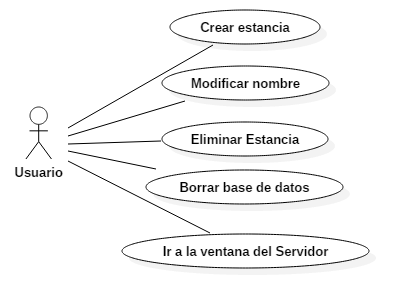
\includegraphics[width=0.7\linewidth]{img/CDUVentanaPrincipal}
	\caption{Funciones que puede realizar el usuario en la ventana principal.}
	\label{fig:CDUVentanaPrincipal}
\end{figure}

\begin{figure}[h!]
	\centering
	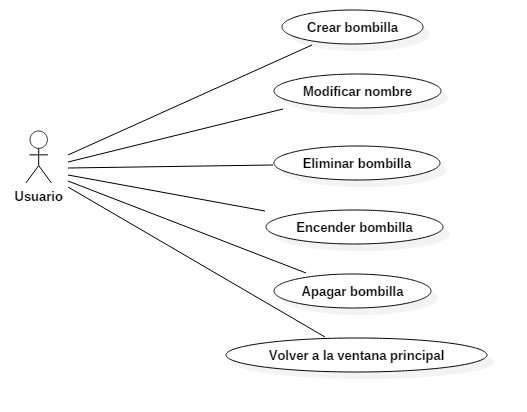
\includegraphics[width=0.9\linewidth]{img/CDUVentanaIluminacion}
	\caption{Funciones que puede realizar el usuario en la ventana de iluminación.}
	\label{fig:CDUVentanaIluminacion}
\end{figure}

\newpage

\begin{figure}[h!]
	\centering
	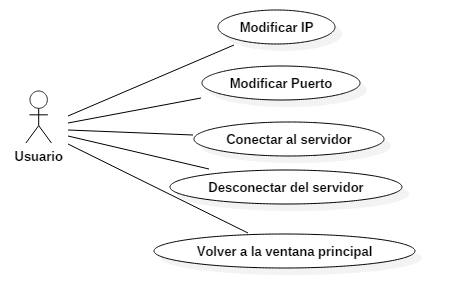
\includegraphics[width=1\linewidth]{img/CDUVentanaServidor}
	\caption{Funciones que puede realizar el usuario en la Ventana del Servidor.}
	\label{fig:CDUVentanaServidor}
\end{figure}

\begin{figure}[h!]
	\centering
	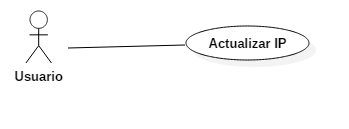
\includegraphics[width=0.8\linewidth]{img/CDUInterfazPython}
	\caption{Funciones que puede realizar el usuario en la interfaz Python.}
	\label{fig:CDUInterfazPython}
\end{figure}

\newpage

\tablaSmallSinColores{Caso de uso ventana principal: \textit{Crear estancia}.}{p{3cm} p{.75cm} p{9.5cm}}{CrearEstancia}{
	\multicolumn{3}{l}{Caso de uso ventana principal: \textit{Crear estancia}.} \\
}
{
	Descripción                            & \multicolumn{2}{p{10.25cm}}{Permite al usuario crear una estancia nueva.} \\\hline
	Requisitos  & \multicolumn{2}{p{10.25cm}}{RF-1} 
	\\\hline
	Precondiciones                         &  \multicolumn{2}{p{10.25cm}}{El usuario debe encontrarse en la ventana principal de la aplicación. \newline Debe estar conectado con el servidor.}   \\\hline
	\multirow{2}{3.5cm}{Secuencia normal}  & Paso & Acción \\\cline{2-3}
	& 1    & El usuario pulsa el botón con símbolo \textbf{+} que se encuentra en la parte superior derecha.
	\\\cline{2-3}
	& 2    & Marca una opción de la lista de estancias en la ventana emergente.
	\\\cline{2-3}
	& 3    & Elige un nombre para esta estancia.
	\\\cline{2-3}
	& 4    & Pulsa sobre el botón \textit{Aceptar} de la ventana emergente.
	\\\hline
	Postcondiciones                        & \multicolumn{2}{p{10.25cm}}{Se ha creado una nueva estancia de ese tipo en la ventana principal.} \\\hline
	Excepciones                        & \multicolumn{2}{p{10.25cm}}{Tratar de crear una estancia sin seleccionar un tipo o escribir un nombre.}\\\hline
	Importancia                            & Alta \\\hline
	Urgencia                               & Alta \\
}

\tablaSmallSinColores{Caso de uso ventana principal: \textit{Modificar nombre}.}{p{3cm} p{.75cm} p{9.5cm}}{ModificarNombreEstancia}{
	\multicolumn{3}{l}{Caso de uso ventana principal: \textit{Modificar nombre}.} \\
}
{
	Descripción                            & \multicolumn{2}{p{10.25cm}}{Permite modificar el nombre de una estancia ya existente.} \\\hline
	Requisitos  & \multicolumn{2}{p{10.25cm}}{RF-2} 
	\\\hline
	Precondiciones                         &  \multicolumn{2}{p{10.25cm}}{El usuario debe encontrarse en la ventana principal de la aplicación. \newline Debe existir al menos una estancia para poder modificar su nombre. \newline Debe estar conectado con el servidor.}   \\\hline
	\multirow{2}{3.5cm}{Secuencia normal}  & Paso & Acción \\\cline{2-3}
	& 1    & Mantener pulsado brevemente sobre la estancia hasta que se muestre el menú contextual.
	\\\cline{2-3}
	& 2    & Seleccionar la opción \textit{Cambiar nombre} del menú contextual.
	\\\cline{2-3}
	& 3    & Escribir el nuevo nombre en la ventana emergente que se nos muestra.
	\\\cline{2-3}
	& 4    & Pulsar sobre el botón \textit{Aceptar} de la ventana emergente.
	\\\hline
	Postcondiciones                        & \multicolumn{2}{p{10.25cm}}{El nombre de la estancia sobre la que estábamos trabajando se ha actualizado.} \\\hline
	Excepciones                        & \multicolumn{2}{p{10.25cm}}{}\\\hline
	Importancia                            & Alta \\\hline
	Urgencia                               & Alta \\
}

\tablaSmallSinColores{Caso de uso ventana principal: \textit{Eliminar estancia}.}{p{3cm} p{.75cm} p{9.5cm}}{EliminarEstancia}{
	\multicolumn{3}{l}{Caso de uso ventana principal: \textit{Eliminar estancia}.} \\
}
{
	Descripción                            & \multicolumn{2}{p{10.25cm}}{Permite eliminar una estancia ya existente.} \\\hline
	Requisitos  & \multicolumn{2}{p{10.25cm}}{RF-3} 
	\\\hline
	Precondiciones                         &  \multicolumn{2}{p{10.25cm}}{El usuario debe encontrarse en la ventana principal de la aplicación. \newline Debe existir al menos una estancia para poder eliminar. \newline Debe estar conectado con el servidor.}   \\\hline
	\multirow{2}{3.5cm}{Secuencia normal}  & Paso & Acción \\\cline{2-3}
	& 1    & Mantener pulsado brevemente sobre la estancia hasta que se muestre el menú contextual.
	\\\cline{2-3}
	& 2    & Seleccionar la opción \textit{Borrar} del menú contextual.
	\\\cline{2-3}
	& 3    & Pulsar sobre el botón \textit{Aceptar} de la ventana emergente de confirmación.
	\\\hline
	Postcondiciones                        & \multicolumn{2}{p{10.25cm}}{La estancia debe desaparecer de la vista actual} \\\hline
	Excepciones                        & \multicolumn{2}{p{10.25cm}}{}\\\hline
	Importancia                            & Alta \\\hline
	Urgencia                               & Alta \\
}

\tablaSmallSinColores{Caso de uso ventana principal: \textit{Borrar base de datos}.}{p{3cm} p{.75cm} p{9.5cm}}{BorrarBaseDeDatos}{
	\multicolumn{3}{l}{Caso de uso ventana principal: \textit{Borrar base de datos}.} \\
}
{
	Descripción                            & \multicolumn{2}{p{10.25cm}}{Permite borrar tanto la base de datos local como la del servidor.} \\\hline
	Requisitos  & \multicolumn{2}{p{10.25cm}}{RF-4} 
	\\\hline
	Precondiciones                         &  \multicolumn{2}{p{10.25cm}}{El usuario debe encontrarse en la ventana principal de la aplicación. \newline Debe estar conectado con el servidor.}   \\\hline
	\multirow{2}{3.5cm}{Secuencia normal}  & Paso & Acción \\\cline{2-3}
	& 1    & Pulsar sobre las tres líneas blancas horizontales de la parte superior izquierda para mostrar el menú desplegable.
	\\\cline{2-3}
	& 2    & Seleccionar la opción \textit{Borrar base de datos} del menú desplegable.
	\\\cline{2-3}
	& 3    & Pulsar sobre el botón \textit{Aceptar} de la ventana emergente de confirmación.
	\\\hline
	Postcondiciones                        & \multicolumn{2}{p{10.25cm}}{Debe borrarse la base de datos local y del servidor.\newline Deben desaparecer todas las estancias que hubiese en la vista.} \\\hline
	Excepciones                        & \multicolumn{2}{p{10.25cm}}{}\\\hline
	Importancia                            & Media \\\hline
	Urgencia                               & Media \\
}

\tablaSmallSinColores{Caso de uso ventana principal: \textit{Ir a la ventana del Servidor}.}{p{3cm} p{.75cm} p{9.5cm}}{ventanaServidor}{
	\multicolumn{3}{l}{Caso de uso ventana principal: \textit{Ir a la ventana del Servidor}.} \\
}
{
	Descripción                            & \multicolumn{2}{p{10.25cm}}{Permite cambiar desde la ventana principal a la ventana del Servidor.} \\\hline
	Requisitos  & \multicolumn{2}{p{10.25cm}}{RF-5} 
	\\\hline
	Precondiciones                         &  \multicolumn{2}{p{10.25cm}}{El usuario debe encontrarse en la ventana principal de la aplicación.}   \\\hline
	\multirow{2}{3.5cm}{Secuencia normal}  & Paso & Acción \\\cline{2-3}
	& 1    & Pulsar sobre las tres líneas blancas horizontales de la parte superior izquierda para mostrar el menú desplegable.
	\\\cline{2-3}
	& 2    & Seleccionar la opción \textit{Servidor} del menú desplegable.
	\\\hline
	Postcondiciones                        & \multicolumn{2}{p{10.25cm}}{Deberá encontrarse en la ventana del Servidor} \\\hline
	Excepciones                        & \multicolumn{2}{p{10.25cm}}{}\\\hline
	Importancia                            & Alta \\\hline
	Urgencia                               & Media \\
}

\tablaSmallSinColores{Caso de uso ventana de iluminación: \textit{Crear bombilla}.}{p{3cm} p{.75cm} p{9.5cm}}{CrearBombilla}{
	\multicolumn{3}{l}{Caso de uso ventana de iluminación: \textit{Crear bombilla}.} \\
}
{
	Descripción                            & \multicolumn{2}{p{10.25cm}}{Permite al usuario crear una bombilla nueva.} \\\hline
	Requisitos  & \multicolumn{2}{p{10.25cm}}{RF-1} 
	\\\hline
	Precondiciones                         &  \multicolumn{2}{p{10.25cm}}{El usuario debe encontrarse en la ventana de iluminación de la aplicación. \newline Debe estar conectado con el servidor.}   \\\hline
	\multirow{2}{3.5cm}{Secuencia normal}  & Paso & Acción \\\cline{2-3}
	& 1    & El usuario pulsa el botón con símbolo \textbf{+} que se encuentra en la parte superior derecha.
	\\\cline{2-3}
	& 2    & Marca la única opción existente en la ventana emergente.
	\\\cline{2-3}
	& 3    & Elige un nombre para esta bombilla.
	\\\cline{2-3}
	& 4    & Pulsa sobre el botón \textit{Aceptar} de la ventana emergente.
	\\\hline
	Postcondiciones                        & \multicolumn{2}{p{10.25cm}}{Se ha creado una nueva bombilla en la ventana de iluminación.} \\\hline
	Excepciones                        & \multicolumn{2}{p{10.25cm}}{Tratar de crear una bombilla sin seleccionarla en la lista o escribir un nombre.}\\\hline
	Importancia                            & Alta \\\hline
	Urgencia                               & Alta \\
}

\tablaSmallSinColores{Caso de uso ventana de iluminación: \textit{Modificar nombre}.}{p{3cm} p{.75cm} p{9.5cm}}{ModificarNombreBombilla}{
	\multicolumn{3}{l}{Caso de uso ventana de iluminación: \textit{Modificar nombre}.} \\
}
{
	Descripción                            & \multicolumn{2}{p{10.25cm}}{Permite modificar el nombre de una bombilla ya existente.} \\\hline
	Requisitos  & \multicolumn{2}{p{10.25cm}}{RF-2} 
	\\\hline
	Precondiciones                         &  \multicolumn{2}{p{10.25cm}}{El usuario debe encontrarse en la ventana de iluminación de la aplicación. \newline Debe existir al menos una bombilla para poder modificar su nombre. \newline Debe estar conectado con el servidor.}   \\\hline
	\multirow{2}{3.5cm}{Secuencia normal}  & Paso & Acción \\\cline{2-3}
	& 1    & Mantener pulsado brevemente sobre la bombilla hasta que se muestre el menú contextual.
	\\\cline{2-3}
	& 2    & Seleccionar la opción \textit{Cambiar nombre} del menú contextual.
	\\\cline{2-3}
	& 3    & Escribir el nuevo nombre en la ventana emergente que se nos muestra.
	\\\cline{2-3}
	& 4    & Pulsar sobre el botón \textit{Aceptar} de la ventana emergente.
	\\\hline
	Postcondiciones                        & \multicolumn{2}{p{10.25cm}}{El nombre de la bombilla sobre la que estábamos trabajando se ha actualizado.} \\\hline
	Excepciones                        & \multicolumn{2}{p{10.25cm}}{}\\\hline
	Importancia                            & Alta \\\hline
	Urgencia                               & Alta \\
}

\tablaSmallSinColores{Caso de uso ventana de iluminación: \textit{Eliminar bombilla}.}{p{3cm} p{.75cm} p{9.5cm}}{EliminarBombilla}{
	\multicolumn{3}{l}{Caso de uso ventana de iluminación: \textit{Eliminar bombilla}.} \\
}
{
	Descripción                            & \multicolumn{2}{p{10.25cm}}{Permite eliminar una bombilla ya existente.} \\\hline
	Requisitos  & \multicolumn{2}{p{10.25cm}}{RF-3} 
	\\\hline
	Precondiciones                         &  \multicolumn{2}{p{10.25cm}}{El usuario debe encontrarse en la ventana de iluminación de la aplicación. \newline Debe existir al menos una bombilla para poder eliminar. \newline Debe estar conectado con el servidor.}   \\\hline
	\multirow{2}{3.5cm}{Secuencia normal}  & Paso & Acción \\\cline{2-3}
	& 1    & Mantener pulsado brevemente sobre la bombilla hasta que se muestre el menú contextual.
	\\\cline{2-3}
	& 2    & Seleccionar la opción \textit{Borrar} del menú contextual.
	\\\cline{2-3}
	& 3    & Pulsar sobre el botón \textit{Aceptar} de la ventana emergente de confirmación.
	\\\hline
	Postcondiciones                        & \multicolumn{2}{p{10.25cm}}{La bombilla debe desaparecer de la vista actual.} \\\hline
	Excepciones                        & \multicolumn{2}{p{10.25cm}}{}\\\hline
	Importancia                            & Alta \\\hline
	Urgencia                               & Alta \\
}

\tablaSmallSinColores{Caso de uso ventana de iluminación: \textit{Encender bombilla}.}{p{3cm} p{.75cm} p{9.5cm}}{EncenderBombilla}{
	\multicolumn{3}{l}{Caso de uso ventana de iluminación: \textit{Encender bombilla}.} \\
}
{
	Descripción                            & \multicolumn{2}{p{10.25cm}}{Permite cambiar el estado de la bombilla a \textit{Encendida}} \\\hline
	Requisitos  & \multicolumn{2}{p{10.25cm}}{RF-4} 
	\\\hline
	Precondiciones                         &  \multicolumn{2}{p{10.25cm}}{El usuario debe encontrarse en la ventana de iluminación de la aplicación. \newline Debe existir al menos una bombilla para poder encenderla. \newline El interruptor deben estar apagado. \newline Debe estar conectado con el servidor.}   \\\hline
	\multirow{2}{3.5cm}{Secuencia normal}  & Paso & Acción \\\cline{2-3}
	& 1    & Pulsar el interruptor de la bombilla para cambiar su estado y encenderla.
	\\\hline
	Postcondiciones                        & \multicolumn{2}{p{10.25cm}}{La bombilla debe encenderse, cambiando su imagen y su estado.} \\\hline
	Excepciones                        & \multicolumn{2}{p{10.25cm}}{}\\\hline
	Importancia                            & Alta \\\hline
	Urgencia                               & Alta \\
}

\tablaSmallSinColores{Caso de uso ventana de iluminación: \textit{Apagar bombilla}.}{p{3cm} p{.75cm} p{9.5cm}}{ApagarBombilla}{
	\multicolumn{3}{l}{Caso de uso ventana de iluminación: \textit{Apagar bombilla}.} \\
}
{
	Descripción                            & \multicolumn{2}{p{10.25cm}}{Permite cambiar el estado de la bombilla a \textit{Apagada}} \\\hline
	Requisitos  & \multicolumn{2}{p{10.25cm}}{RF-5}
	\\\hline
	Precondiciones                         &  \multicolumn{2}{p{10.25cm}}{El usuario debe encontrarse en la ventana de iluminación de la aplicación. \newline Debe existir al menos una bombilla para poder apagarla. \newline El interruptor deben estar encendido. \newline Debe estar conectado con el servidor.}   \\\hline
	\multirow{2}{3.5cm}{Secuencia normal}  & Paso & Acción \\\cline{2-3}
	& 1    & Pulsar el interruptor de la bombilla para cambiar su estado y apagarla.
	\\\hline
	Postcondiciones                        & \multicolumn{2}{p{10.25cm}}{La bombilla debe apagarse, cambiando su imagen y su estado.} \\\hline
	Excepciones                        & \multicolumn{2}{p{10.25cm}}{}\\\hline
	Importancia                            & Alta \\\hline
	Urgencia                               & Alta \\
}

\tablaSmallSinColores{Caso de uso ventana de iluminación: \textit{Volver a la ventana principal}.}{p{3cm} p{.75cm} p{9.5cm}}{volverVentanaPrincipal}{
	\multicolumn{3}{l}{Caso de uso ventana de iluminación: \textit{Volver a la ventana principal}.} \\
}
{
	Descripción                            & \multicolumn{2}{p{10.25cm}}{Permite ir desde la ventana de iluminación a la ventana principal.} \\\hline
	Requisitos  & \multicolumn{2}{p{10.25cm}}{RF-6} 
	\\\hline
	Precondiciones                         &  \multicolumn{2}{p{10.25cm}}{El usuario debe encontrarse en la ventana de iluminación de la aplicación.}   \\\hline
	\multirow{2}{3.5cm}{Secuencia normal}  & Paso & Acción \\\cline{2-3}
	& 1    & Pulsar sobre la flecha que se encuentra en la parte superior izquierda.
	\\\hline
	Postcondiciones                        & \multicolumn{2}{p{10.25cm}}{Nos encontramos en la ventana principal.} \\\hline
	Excepciones                        & \multicolumn{2}{p{10.25cm}}{}\\\hline
	Importancia                            & Media \\\hline
	Urgencia                               & Media \\
}



\tablaSmallSinColores{Caso de uso ventana del Servidor: \textit{Modificar IP}.}{p{3cm} p{.75cm} p{9.5cm}}{ModificarIP}{
	\multicolumn{3}{l}{Caso de uso ventana del Servidor: \textit{Modificar IP}.} \\
}
{
	Descripción                            & \multicolumn{2}{p{10.25cm}}{Actualiza el valor asignado a la IP del servidor.} \\\hline
	Requisitos  & \multicolumn{2}{p{10.25cm}}{RF-1} 
	\\\hline
	Precondiciones                         &  \multicolumn{2}{p{10.25cm}}{El usuario debe encontrarse en la ventana de servidor de la aplicación.}   \\\hline
	\multirow{2}{3.5cm}{Secuencia normal}  & Paso & Acción \\\cline{2-3}
	& 1    & Pulsar sobre el campo de texto de la IP.
	\\\cline{2-3}
	& 2    & Escribir la nueva IP que se quiera utilizar.
	\\\cline{2-3}
	& 3    & Pulsar sobre el botón \textit{Actualizar}.
	\\\hline
	Postcondiciones                        & \multicolumn{2}{p{10.25cm}}{La IP ha sido guardada en la base de datos.} \\\hline
	Excepciones                        & \multicolumn{2}{p{10.25cm}}{}\\\hline
	Importancia                            & Alta \\\hline
	Urgencia                               & Alta \\
}

\tablaSmallSinColores{Caso de uso ventana del Servidor: \textit{Modificar Puerto}.}{p{3cm} p{.75cm} p{9.5cm}}{ModificarPuerto}{
	\multicolumn{3}{l}{Caso de uso ventana del Servidor: \textit{Modificar Puerto}.} \\
}
{
	Descripción                            & \multicolumn{2}{p{10.25cm}}{Actualiza el valor asignado a la IP del servidor.} \\\hline
	Requisitos  & \multicolumn{2}{p{10.25cm}}{RF-2} 
	\\\hline
	Precondiciones                         &  \multicolumn{2}{p{10.25cm}}{El usuario debe encontrarse en la ventana de servidor de la aplicación.}   \\\hline
	\multirow{2}{3.5cm}{Secuencia normal}  & Paso & Acción \\\cline{2-3}
	& 1    & Pulsar sobre el campo de texto del Puerto.
	\\\cline{2-3}
	& 2    & Escribir el nuevo Puerto que se quiera utilizar.
	\\\cline{2-3}
	& 3    & Pulsar sobre el botón \textit{Actualizar}.
	\\\hline
	Postcondiciones                        & \multicolumn{2}{p{10.25cm}}{El Puerto se guarda en la base de datos.} \\\hline
	Excepciones                        & \multicolumn{2}{p{10.25cm}}{}\\\hline
	Importancia                            & Alta \\\hline
	Urgencia                               & Alta \\
}

\tablaSmallSinColores{Caso de uso ventana del Servidor: \textit{Conectar al servidor}.}{p{3cm} p{.75cm} p{9.5cm}}{ConectarAlServidor}{
	\multicolumn{3}{l}{Caso de uso ventana del Servidor: \textit{Conectar al servidor}.} \\
}
{
	Descripción                            & \multicolumn{2}{p{10.25cm}}{Crea una conexión con el Servidor.} \\\hline
	Requisitos  & \multicolumn{2}{p{10.25cm}}{RF-3} 
	\\\hline
	Precondiciones                         &  \multicolumn{2}{p{10.25cm}}{El usuario debe encontrarse en la ventana de servidor de la aplicación.\newline El campo IP debe contener una IP válida. \newline El campo Puerto debe contener un puerto válido.}   \\\hline
	\multirow{2}{3.5cm}{Secuencia normal}  & Paso & Acción \\\cline{2-3}
	& 1    & Pulsar el botón \textit{Conectar}.
	\\\hline
	Postcondiciones                        & \multicolumn{2}{p{10.25cm}}{El estado del servidor pasa a \textit{Conectado}.} \\\hline
	Excepciones                        & \multicolumn{2}{p{10.25cm}}{}\\\hline
	Importancia                            & Alta \\\hline
	Urgencia                               & Alta \\
}

\tablaSmallSinColores{Caso de uso ventana del Servidor: \textit{Desconectar del servidor}.}{p{3cm} p{.75cm} p{9.5cm}}{DesconectarDelServidor}{
	\multicolumn{3}{l}{Caso de uso ventana de servidor: \textit{Desconectar del servidor}.} \\
}
{
	Descripción                            & \multicolumn{2}{p{10.25cm}}{Cierra una conexión existente con el Servidor.} \\\hline
	Requisitos  & \multicolumn{2}{p{10.25cm}}{RF-4} 
	\\\hline
	Precondiciones                         &  \multicolumn{2}{p{10.25cm}}{El usuario debe encontrarse en la ventana del Servidor de la aplicación.\newline Debe existir una conexión con el Servidor actualmente.}   \\\hline
	\multirow{2}{3.5cm}{Secuencia normal}  & Paso & Acción \\\cline{2-3}
	& 1    & Pulsar el botón \textit{Desconectar}.
	\\\hline
	Postcondiciones                        & \multicolumn{2}{p{10.25cm}}{El estado del servidor pasa a \textit{Desconectado}.} \\\hline
	Excepciones                        & \multicolumn{2}{p{10.25cm}}{}\\\hline
	Importancia                            & Alta \\\hline
	Urgencia                               & Alta \\
}

\tablaSmallSinColores{Caso de uso ventana del Servidor: \textit{Volver a la ventana principal}.}{p{3cm} p{.75cm} p{9.5cm}}{volverVentanaPrincipalServidor}{
	\multicolumn{3}{l}{Caso de uso ventana del Servidor: \textit{Volver a la ventana principal}.} \\
}
{
	Descripción                            & \multicolumn{2}{p{10.25cm}}{Permite ir desde la ventana del Servidor a la ventana principal.} \\\hline
	Requisitos  & \multicolumn{2}{p{10.25cm}}{RF-5} 
	\\\hline
	Precondiciones                         &  \multicolumn{2}{p{10.25cm}}{El usuario debe encontrarse en la ventana del Servidor de la aplicación.}   \\\hline
	\multirow{2}{3.5cm}{Secuencia normal}  & Paso & Acción \\\cline{2-3}
	& 1    & Pulsar sobre la flecha que se encuentra en la parte superior izquierda.
	\\\hline
	Postcondiciones                        & \multicolumn{2}{p{10.25cm}}{Nos encontramos en la ventana principal} \\\hline
	Excepciones                        & \multicolumn{2}{p{10.25cm}}{}\\\hline
	Importancia                            & Media \\\hline
	Urgencia                               & Media \\
}

\tablaSmallSinColores{Caso de uso Interfaz Python: \textit{Actualizar IP}.}{p{3cm} p{.75cm} p{9.5cm}}{ActualizarIPPython}{
	\multicolumn{3}{l}{Caso de uso Interfaz Python: \textit{Actualizar IP}.} \\
}                                                        
{
	Descripción                            & \multicolumn{2}{p{10.25cm}}{Permite introducir una IP nueva.} \\\hline
	Requisitos  & \multicolumn{2}{p{10.25cm}}{RF-1} 
	\\\hline
	Precondiciones                         &  \multicolumn{2}{p{10.25cm}}{El usuario debe encontrarse en la Interfaz Python del Servidor tras arrancar el Servidor.\newline La IP debe estar vacía o incorrecta.}   \\\hline
	\multirow{2}{3.5cm}{Secuencia normal}  & Paso & Acción \\\cline{2-3}
	& 1    & En el error que se muestre, pulsar el botón \textit{Aceptar}.
	\\\cline{2-3}
	& 2    & En la nueva ventana que se abrirá, escribir la nueva IP en el cuadro de texto correspondiente.
	\\\cline{2-3}
	& 3    & Pulsar el botón \textit{Actualizar}.
	\\\hline
	Postcondiciones                        & \multicolumn{2}{p{10.25cm}}{El socket estará escuchando correctamente en esa IP.} \\\hline
	Excepciones                        & \multicolumn{2}{p{10.25cm}}{}\\\hline
	Importancia                            & Alta \\\hline
	Urgencia                               & Alta \\
}